\section{ILLUSTRATIONS, GRAPHS, AND PHOTOGRAPHS}
\label{sec:illust}

The purpose of this experiment is to implement our generalized critic instead of a regular critic on top of previously known state-of-the-art algorithms and check empirically the effect this has on their performance while paying particular attention to :
\begin{enumerate}
\item the tasks, and whether different environments react differently to this change in implementation;
\item the 
\end{enumerate}

We will then provide an interpretation of the results and try to explain 

\subsection{Experiment Setting}
% In the case of a continuous action space, $\pi$ is a gaussian distribution. <- add this to experiments
For the sake of this experiment, we consider four continuous control tasks of the OpenAI Gym toolkit collection: 2D Walker, Inverted Pendulum, Ant and Half Cheetah. 
We implement our Generalized Critic on top of a PPO-Clip Actor \cite{ppo}.
\begin{itemize}
\item performance (average return) of base algorithms in every task,
\item performance with four versions of Generalized Critic: two different values of lambda and gamma and the possible combinations with two values of the weights of the linear combination.
\end{itemize}

\subsection{Policy Optimization}

The policy optimization method that we use for this experiment is a Proximal Policy Optimization with the Clip variant. 

%present ppo

\subsection{Trained Tasks}



\subsection{Experiment Results}

\begin{tabular}{c}

\end{tabular}
% Below is an example of how to insert images. Delete the ``\vspace'' line,
% uncomment the preceding line ``\centerline...'' and replace ``imageX.ps''
% with a suitable PostScript file name.
% -------------------------------------------------------------------------
\begin{figure}[htb]

\begin{minipage}[b]{1.0\linewidth}
  \centering
  \centerline{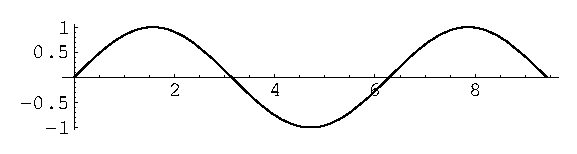
\includegraphics[width=8.5cm]{images/image1}}
%  \vspace{2.0cm}
  \centerline{(a) Result 1}\medskip
\end{minipage}
%
\begin{minipage}[b]{.48\linewidth}
  \centering
  \centerline{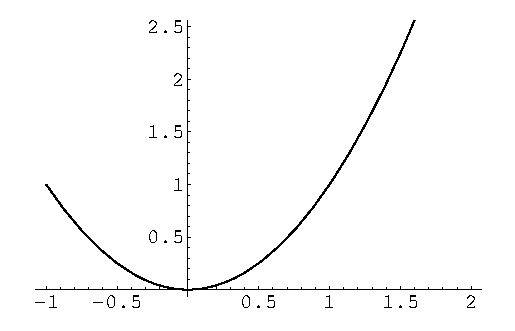
\includegraphics[width=4.0cm]{images/image3}}
%  \vspace{1.5cm}
  \centerline{(b) Results 3}\medskip
\end{minipage}
\hfill
\begin{minipage}[b]{0.48\linewidth}
  \centering
  \centerline{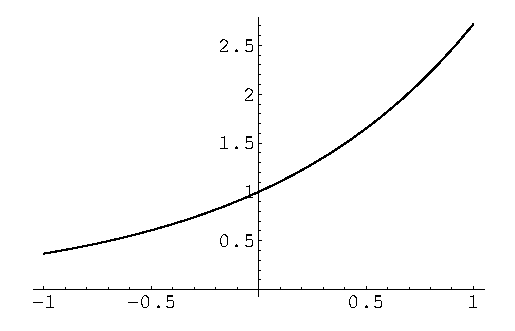
\includegraphics[width=4.0cm]{images/image4}}
%  \vspace{1.5cm}
  \centerline{(c) Result 4}\medskip
\end{minipage}
%
\caption{Example of placing a figure with experimental results.}
\label{fig:res}
%
\end{figure}


% To start a new column (but not a new page) and help balance the last-page
% column length use \vfill\pagebreak.
% -------------------------------------------------------------------------
%\vfill
%\pagebreak

